Im Versuch wurden S11 Messungen von einem BNC- und einem SMA-Kabel durchgeführt sowie deren
Verkürzungsfaktor bestimmt.

\begin{figure}[h]
  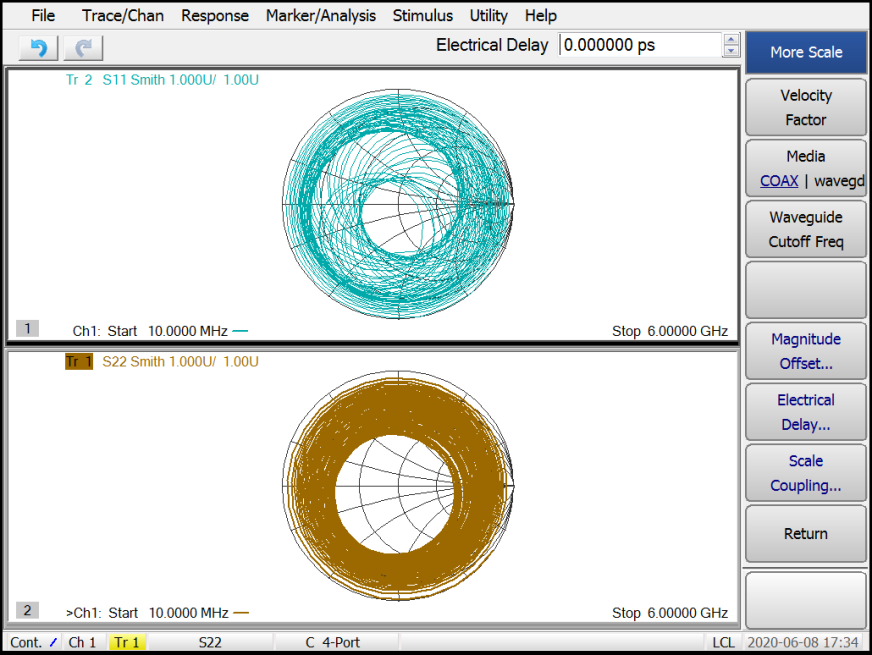
\includegraphics[width=\textwidth]{2_5}
  \caption{S11/S22 Messung von BNC (S11, blau) und SMA (S22, braun) im
    Smithdiagramm, offener Abschluss}
  \label{fig:circly}
\end{figure}

\begin{figure}[h]
  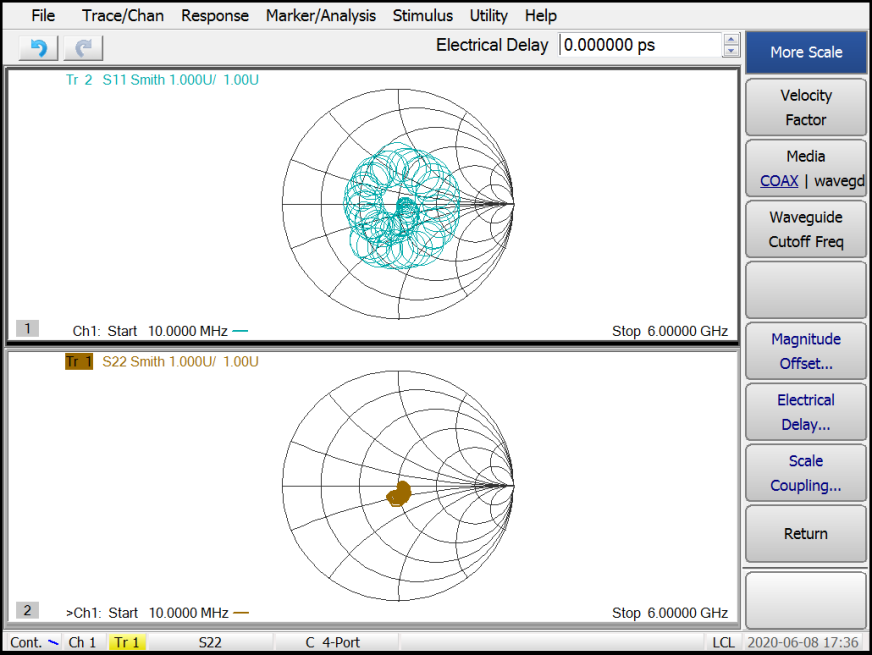
\includegraphics[width=\textwidth]{2_5_zusamme}
  \caption{S11/S22 Messung von BNC (S11, blau) und SMA (S22, braun) im
    Smithdiagramm, Abschluss}
  \label{fig:circly_load}
\end{figure}

Qualitativ kann aus dem Smithdiagramm Abb. \ref{fig:circly} erkannt werden, dass
der Reflexionsfaktor des BNC-Kabels deutlich frequenzabhängiger ist, als der des
SMA-Kabels.

Bei der Transmissionsmessung über S31 bzw. S42 wurde der zweite Port
verbunden und somit die Leitung abgeschlossen, die Auswirkung auf den
Reflexionsfaktor sieht man in Abb. \ref{fig:circly_load}. Das BNC-Kabel weist
auch hier noch einen sehr frequenzabhängigen und hohen Reflexionsfaktor im
gemssenen Frequenzbereich auf. Die Messung der Transmission ergab Abb.
\ref{fig:trans}. Auch bei der Transmission (Übertragungsfunktion) erkennt man
einen weniger linearen Verlauf des BNC-Kabels, was in Bezug auf die Güte einen
Nachteil gegenüber der SMA-Leitung darstell, was in Bezug auf die Güte einen
Nachteil gegenüber der SMA-Leitung darstelltt.

\begin{figure}[h]
  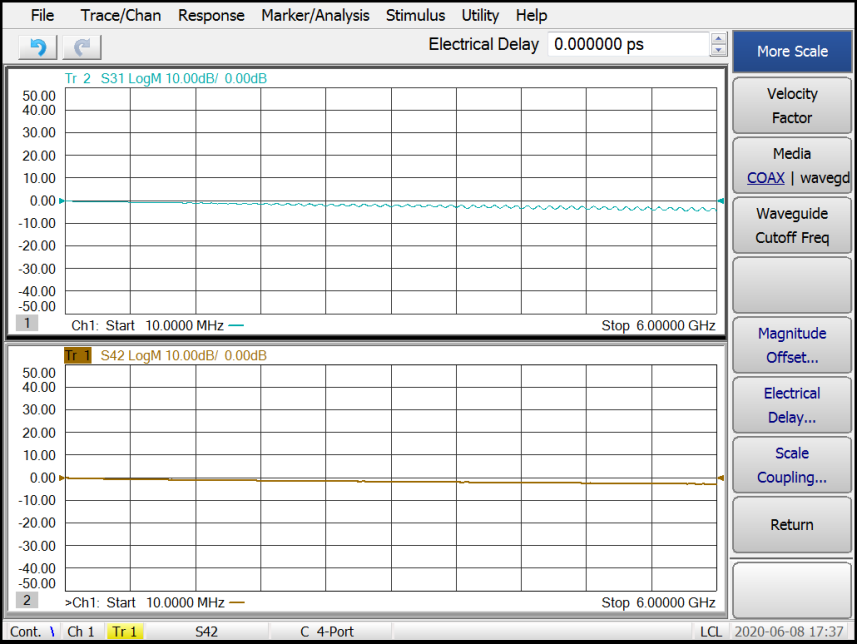
\includegraphics[width=\textwidth]{2_5_trans}
  \caption{Transmissionmessung von SMA und BNC} 
  \label{fig:circly_load}
\end{figure}

\begin{figure}[h]
  \begin{center}
  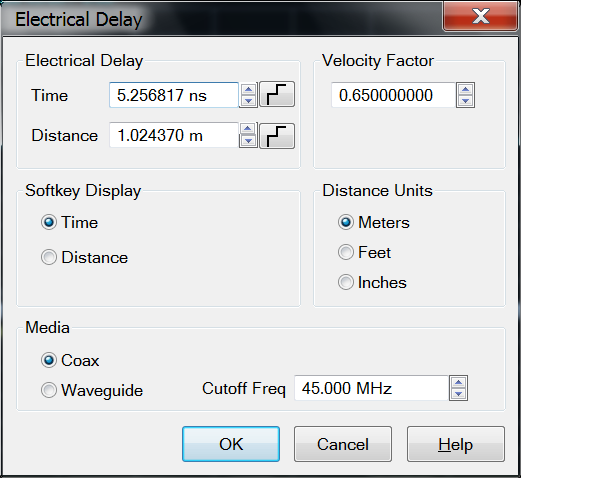
\includegraphics[width=0.618\textwidth]{BNC_lange}
  \end{center}
  \caption{Bestimmung des BNC-Verkürzungsfaktors}
  \label{fig:BNC_lange}
\end{figure}
\begin{figure}[h]
  \begin{center}
  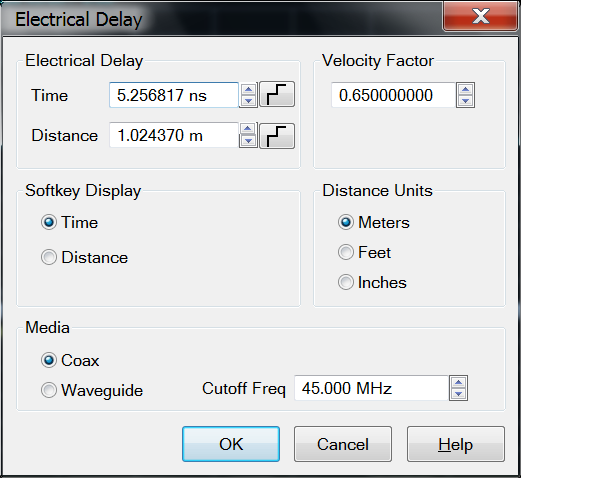
\includegraphics[width=0.618\textwidth]{BNC_lange}
  \end{center}
  \caption{Bestimmung des SMA-Verkürzungsfaktors}
  \label{fig:SMA_lange}
\end{figure}

Die Bestimmung des Verkürzungsfaktors der Leitungen erfolgte mithilfe der
Softwarelösung des Netzwerkanalysators, ähnlich zu der Methode aus der
vorherigen Aufgabe beim Dämpfungsglied. Das Electrical Delay wurde solange
angepasst, bis die Phase den Wert $0$ annahm. Da die Länge der Leitungen
bekannt war (jeweils $1 \, \si{\meter}$) konnte das Ergebnis für den
Verkürzungsfaktor überprüft werden.






